\documentclass[12pt, a4paper, openany]{book}
\usepackage[italian]{babel}
\usepackage{listings}
\usepackage{graphicx}
\usepackage{fancyvrb}
\graphicspath{ {./images/} }

\begin{document}
\title{PES - Probabilità e Statistica per l'informatica}
\author{Elia Ronchetti}
\date{Marzo 2022}

\maketitle
\tableofcontents
\chapter{Introduzione}
Il corso di probabilità e statistica per l'informatica è diviso in 2 parti
\begin{enumerate}
    \item Stastica Descrittiva - Descrivere e riassumere i dati
    \begin{enumerate}
        \item Probabilità - Descrivere matematicamente i fenomeni casuali
    \end{enumerate}
    \item Statistica inferenziale - Trarre conclusioni dai dati
\end{enumerate}

\chapter{Analisi Descrittiva}
\section{Descrivere i dati}
Per descrivere una raccolta dati in maniera chiara e immediata è utile utilizzare una \textbf{tabella delle frequenze}
all'interno della quale sono contenuti:
\begin{itemize}
    \item Valori
    \item Frequenze Assolute - Numero di volte in cui compare "i" nell'insieme di dati
    \item Frequenze Relative - Frazione di volte in cui compare i nell'insieme di dati
    \item Percentuali - (Frequenza relativa x 100)
\end{itemize}

Il dato che compare con frequenza più alta è detto \textbf{moda}.

I dati possono essere
\begin{itemize}
    \item Qualitativi
    \item Quantitativi 
\end{itemize}
Noi useremo i dati \textbf{quantitativi}

\subsection{Rappresentazione dei dati}
Per rappresentare le frequenze (assolute o relative) risulta efficace e immediato l'utilizzo di un grafico a barre detto istogramma,
esso rappresenta in graficamente la tabella, chiaramamente da esso è possibile risalire alla tabella stessa.
Capita di avere degli insiemi di dati che assumono un valore elevato di valori distini, per questo conviene suddividerli in classi e
determinare la frequenza di ciascuna classe. In questo modo c'è una perdita d'informazioni (sui valori specifici), ma così facendo possiamo
calcolare le frequenze delle classi e avere un'idea migliore della distribuzione dei dati.

\subsection{Dati Bivariati}
Quando per ciascun individuo vengono misurate due variabili ci troviamo un insieme di N dati a coppie detti \textbf{dati bivariati}.
Anche in questo caso è possibile calcolare le frequenze, in questo caso detto \textbf{frequenze congiunte}.

è possibile, inoltre, misurare la correlazione tra le due variabili attraverso per esempio un diagramma di dispersione (detto anche scatterplot).

\paragraph{Correlazione non significa causalità!} Non è detto che l'aumento di una variabile causi la diminuzione dell'altra o viceversa, potrebbe esserci una causa comune. 

\section{Riassumere i dati}
Dopo aver rappresentato i dati vogliamo ora riassumerli mediante quantità numeriche, dette \textbf{Statistiche Campionarie}, al fine di sintetizzare le proprietà
salienti dei dati.

\subsection{Indici di posizione}
Per definire il centro dell'insieme dei dati definiamo la 
\paragraph{\textbf{Media Campionaria}} \scalebox{2}{$\frac{x_1 + x_2 + \dots + x_n}{N}$} %Aggiungere sommatoria

Per misurare il valore in posizione centrale (considerando l'insieme di dati ordinato), utilizziamo la
\paragraph{\textbf{Mediana}}
\begin{itemize}
    \item Se N dispari - {$X_\frac{N+1}{2}$}
    \item Se N pari - $m = \frac{x_\frac{N}{2}+x_(\frac{N}{2}+1)}{2}$
\end{itemize}

La mediana è insesibile alle code

\section{Coefficiente di correlazione lineare}
Posso misurare il grado di correlazione tra una coppia di dati attraverso il coefficiente di correlazione lineare. 

\begin{equation}
    r = \frac{\sum_{k=1}^N (x_i - x)(y_i - y)}{(N -1)S_x S_y}
\end{equation}

Si può mostrare che:
\begin{equation}
    -1<=r<=1
\end{equation}

In generale $r > 0$ indica una correlazione positiva
\\ $r < 0$ indica una correlazione negativa 

\subsection{Correlazioni significative}
$|r| > 0.7$ Correlazione significativa
\\$|r| < 0.3$ Correlazione debole

\section{Percentili e quantili}
Per analizzare la distribuzione dei dati è utile fissare un numero k che rappresenta la posizione all'interno dato all'interno dell'insieme
questo valore percentuale è detto \textbf{k-esimo Percentile Campionario}, valore t per cui
\begin{itemize}
    \item almeno il k\% dei dati è $ <= t$
    \item almeno il $(100 -k)\%$ dei dati è $<= t$
\end{itemize}

I casi più importanti sono per k = 25, 50, 75
\\ Risulta pratico scrivere $k = 100p$ dove $p = \frac{k}{100}\in [0, 1]$, dove i casi importanti sono per:
\begin{itemize} 
    \item $p = \frac{1}{4}: k = 100p$ = 25-esimo percentile = primo quartile $q_1$
    \item $p = \frac{1}{2}: k = 100p$ = 50-esimo percentile = secondo quartile $q_2$ = mediana m
    \item $p = \frac{3}{4}: k = 100p$ = 75-esimo percentile = terzo quartile $q_3$
\end{itemize}

Per calcolare il k-esimo percentile t è necessario:
\begin{enumerate}
    \item Ordinare l'insieme di dati $x_1 <= x_2 <= \dots <= x_n$
    \item Se $N_p$ non è intera $t=x_i$ è il dato la cui posizione i è l'intero successivo a $N_p$
    \item Se $N_p$ è intera $t = \frac{x_(Np) x_(Np+1)}{2}$ è la media aritmetica fra il dato in posizione N e il successivo 
\end{enumerate}

\paragraph{Nota per R} Esistono diverse definizioni di quantile, R èer esempio ne utilizza una diversa di default

\'E possibile utilizzare i \textbf{Boxplot} per la rappresentazione dei quantili

\chapter{Probabilità}
Il calcolo delle probabilità è la teoria matematica che permette di descrivere e studiare \textbf{esperimenti aleatori}
\paragraph{Esperimento aleatorio} $\to$ Fenomeno il cui esito non è prevedibile con certezza a priori
\section{Introduzione}
La descrizione matematica si articola in tre passi
\begin{enumerate}
    \item Spazio campionario (o spazio degli esiti)$\to$ Insieme $\Omega$ che contiene tutti i possibili esiti dell'esperimento \\ es. Tiro un dato a sei facce $\Omega = {1, 2, 3, 4, 5, 6}$
    \item Eventi $\to$ sono i sottinsiemi dello spazio campionario $A \subseteq \Omega$ \\ es. Tiro un dado a sei facce: esce un numero pari $A = {2, 4, 6}$
    \item Probabilità $\to$ Regola che assegna, in modo coerente, a ogni evento $A \subseteq \Omega$ un "grado di fiducia" $P(A)$, tra 0 e 1, che attribuiamo al verificarsi di A
    O funzione $P: P(\Omega) \to [0, 1]$ che soddisfa opportune proprietà
\end{enumerate}
\section{Proprietà di base} 
\begin{enumerate}
    \item $P(\Omega) = 1$
    \item Se A e B sono eventi disgiunti, cioè $A \cap B \neq \emptyset$, allora \\ $P (A \cup B) = P(A) + P(B)$
\end{enumerate}
\paragraph{La coppia $(\Omega, P)$ è detta \textbf{Spazio di Probabilità}}.
\\ Fissiamo uno spazio di probabilità $(\Omega, P)$.
Da queste proprietà si deducono molte altre proprietà
\begin{itemize}
    \item $P(\emptyset) = 0$
    \item \textbf{Regola del complementare} $\to P(A^c) = 1 - P(A)$ \\ Vale per ogni A
    \item \textbf{Regola della addizione di probabilità} $\to P(A \cup B) = P(A) + P(B) - P(A \cap B)$ 
    \\ Vale per ogni A, B (anche $A \cap B \neq \emptyset$)
    \item Monotonia: se $A \subseteq B$ allora $P(A) <= P(B)$
\end{itemize}
\paragraph{Analogia} c'è un analogia tra probabilità e area
\\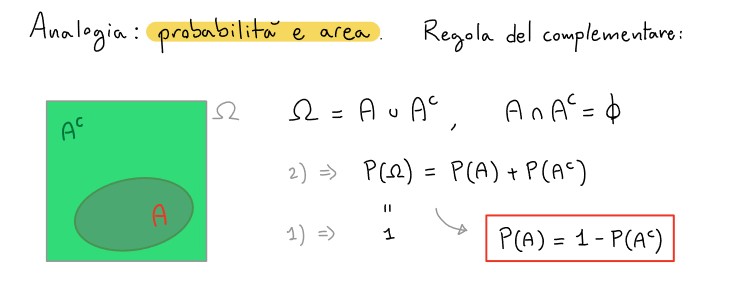
\includegraphics{analogia_prob_area.png}
\section{Calcolo combinatorio}



\chapter{Esame}
L'esame sarà strutturato nella seguente maniera
\paragraph{Parte 1 - Teoria}
8 Domande a risposta multipla - Punteggio 10/30
\paragraph{Parte 2 - Pratica}
4 Esercizi a risposta aperta - Punteggio 20/30
\paragraph{Progetto (facoltativo)}
Progetto R, da consegnare prima dell'esame, può fornire un massimo di 2/30

\end{document}